\documentclass[12pt]{article}
\usepackage[utf8]{inputenc}
\usepackage[T1]{fontenc}
\usepackage[french]{babel}
\usepackage{geometry}
\usepackage{listings}
\usepackage{xcolor}
\usepackage{graphicx}
\usepackage{hyperref}
\usepackage{enumitem}
\usepackage{titlesec}
\usepackage{tocloft}
\usepackage{caption}

\geometry{a4paper, margin=2.5cm}

\lstset{
    basicstyle=\ttfamily,
    backgroundcolor=\color{gray!10},
    frame=single,
    breaklines=true
}

\renewcommand{\cftsecleader}{\cftdotfill{\cftdotsep}}
\setlength{\cftbeforesecskip}{5pt}
\setcounter{tocdepth}{3}

\title{Guide complet de la manipulation de notre application d’aide à l’archivage et à la consultation des projets des étudiants.}
\author{Ange FOKAM}
\date{30/juin/2025}

\begin{document}

\maketitle
\clearpage

\tableofcontents
\newpage
\listoffigures
\clearpage

% -------------------------------
\textbf{\textit{Pour les développeurs et les administrateurs système}}

\rule{\linewidth}{0.2pt}

\section*{À propos du guide :}
\addcontentsline{toc}{section}{À propos du guide}

\begin{itemize}[label=--]
    \item \textbf{Objectif du guide} : Explique comment déployer, manipuler et utiliser l'application.
    \item \textbf{Public cible} : Administrateurs système futurs et développeurs futurs.
    \item \textbf{Structure du document} : Deux sections, une pour le Matériel à disposer et l'autre pour le déploiement technique de l'application.
    \item \textbf{Prérequis généraux} : Accès réseau, identifiants, connaissances de base en informatique et en programmation.
\end{itemize}

\rule{\linewidth}{0.2pt}

        \begin{figure}[h] 
            \centering 
            
\includegraphics[width=0.75\textwidth]{./img/logo1.jpg} 
        \end{figure}

\vfill
\rule{\linewidth}{0.2pt}
\textbf{\textit{Ce guide a pour objectif de rendre l’utilisation et la maintenance de l’application aussi claires et accessibles
que possible. En suivant les étapes décrites, les développeurs pourront exploiter pleinement le système tout en en assurant sa 
pérennité et son efficacité.}}

\newpage

% Introduction
{\fontsize{14}{16}\section*{Introduction}}
\addcontentsline{toc}{section}{Introduction}
Dans le monde du développement, les applications doivent être entretenues au quotidien.
À cet effet, elles doivent être conçues de manière à ce que les générations futures puissent
facilement les maintenir en activité. De plus, le développement des applications doit répondre
aux besoins de leurs utilisateurs.

De ce fait, nous avons mis en place une série d'étapes pour le lancement de notre application
à partir d’un poste personnel, afin de faciliter la compréhension et la maintenance par les
développeurs et administrateurs.

Bien que ce processus puisse sembler complexe, il vise à faciliter la prise en main et la
maintenance à long terme de l’application par les futurs intervenants, ainsi que la gestion
des projets de fin de cycle des étudiants.

Pour un déploiement complet de l'application, nous avons réparti la présentation en cinq
parties : la première présentera le matériel nécessaire, la deuxième expliquera l'installation
des environnements, la troisième montrera comment modifier les variables d'environnement, la
quatrième abordera le déploiement des serveurs, et la cinquième traitera de l'ouverture de l'application.

\vspace{0.5cm}
\rule{\linewidth}{0.2pt}

\newpage
% Guide de déploiement
{\fontsize{14}{16}\section*{Guide de déploiement de l’application}}
\addcontentsline{toc}{section}{Guide de déploiement de l’application}
\setcounter{subsection}{0} % On remet la numérotation des sections à zéro
\renewcommand\thesubsection{\arabic{subsection}}
\rule{\linewidth}{0.2pt}

\subsection{Matériel à disposer et prérequis}

    \subsubsection{Matériel nécessaires :}
    
Avant de commencer l'installation, assurez-vous d'avoir les éléments suivants :
        \begin{itemize}[label=--]
            \item PHP (version 8.0 ou plus récente (8.3 qui est la dernière mise à jour))
            \item Composer (version 2.7 de base )
            \item Angular 17
            \item Laravel 10+
            \item VS Code (de préférence comme éditeur de texte)
            \item MySQL (via XAMPP ou autre) ou MariaDB ou encore PostgreSQL 
            \item Elasticsearch (version compatible avec votre système)
        \end{itemize}
    \rule{\linewidth}{0.2pt}
    \subsubsection{Configuration minimale recommandée :}

Pour ce qui est du matériel et les ressources nécessaires, vous devez procéder au déploiement.

        \begin{itemize}[label=--]
            \item Processeur : 2 GHz double cœur ou plus
            \item RAM : 8 Go minimum, 12Go recommandée
            \item Stockage : 30 Go d’espace libre ou plus
        \end{itemize}
    \rule{\linewidth}{0.2pt}
    \subsubsection{Outils nécessaires :}

        \begin{itemize}[label=--]
            \item Git (avec un compte GitHub pour la collaboration)
            \item Accès à Internet (FAI ou VPN)
            \item Navigateur web à jour (Chrome, Firefox, Edge, Opera, avast-secure-browser etc.)
        \end{itemize}
\rule{\linewidth}{0.2pt}
\subsection{Étapes de déploiement}

Voici les étapes pour l’ouverture du projet (for windows and Linux):

    \subsubsection{Cloner le dépôt GitHub}

Lien du dépôt :
        \begin{lstlisting}
git clone https://github.com/Noobs440/UV_PROJET_AIGLE.git
        \end{lstlisting}
\rule{\linewidth}{0.2pt}
    \subsubsection{Configurer l’environnement}

Créer le fichier `.env` :
        \begin{lstlisting}
cp .env.example .env
        \end{lstlisting}
Ouvrez le fichier .env dans un éditeur de texte et configurez les variables d'environnement suivantes
en modifiant le fichier `.env`:
        \begin{lstlisting}
DB_CONNECTION=mysql
DB_HOST=127.0.0.1
DB_PORT=3306
DB_DATABASE=nom_de_votre_base
DB_USERNAME=nom_utilisateur
DB_PASSWORD=mot_de_passe
        \end{lstlisting}
\rule{\linewidth}{0.2pt}

    \subsubsection{Modification des variables d’environnement}
Dans la barre de recherche de votre pc tapez : "path" ou "variables d'environnement"
        \begin{figure}[h] 
            \centering 
            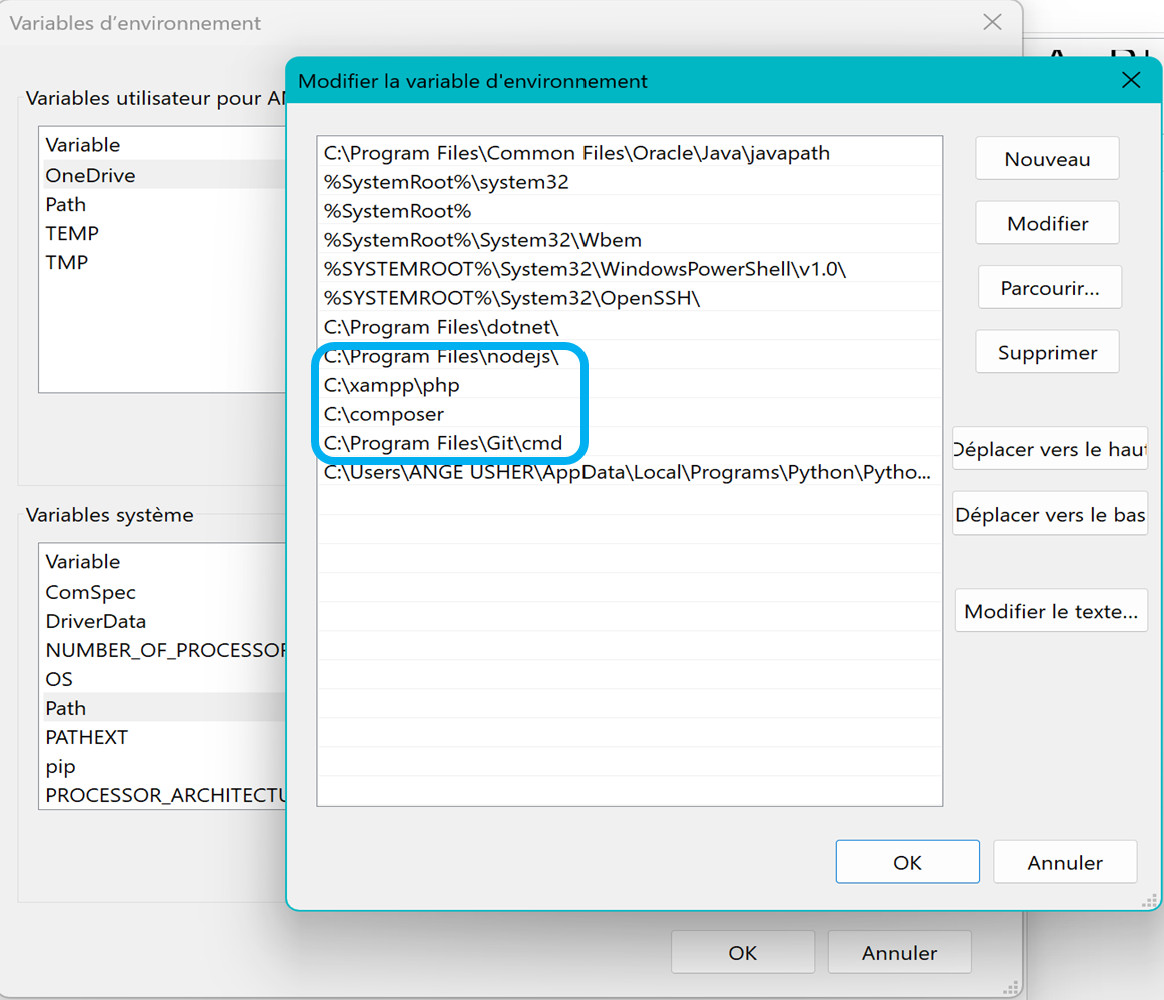
\includegraphics[width=0.70\textwidth]{./img/path.png} 
            \caption{Chemin d'accès aux variables d’environnement système}
        \end{figure}

\rule{\linewidth}{0.2pt}
    \subsubsection{Générer la clé d'application}

Générez une nouvelle clé d'application en exécutant la commande suivante :
        \begin{lstlisting}
php artisan key:generate
        \end{lstlisting}
\rule{\linewidth}{0.2pt}

    \subsubsection{Configurer XAMPP et lancer Apache + MySQL}
        \begin{figure}[h!] 
            \centering 
            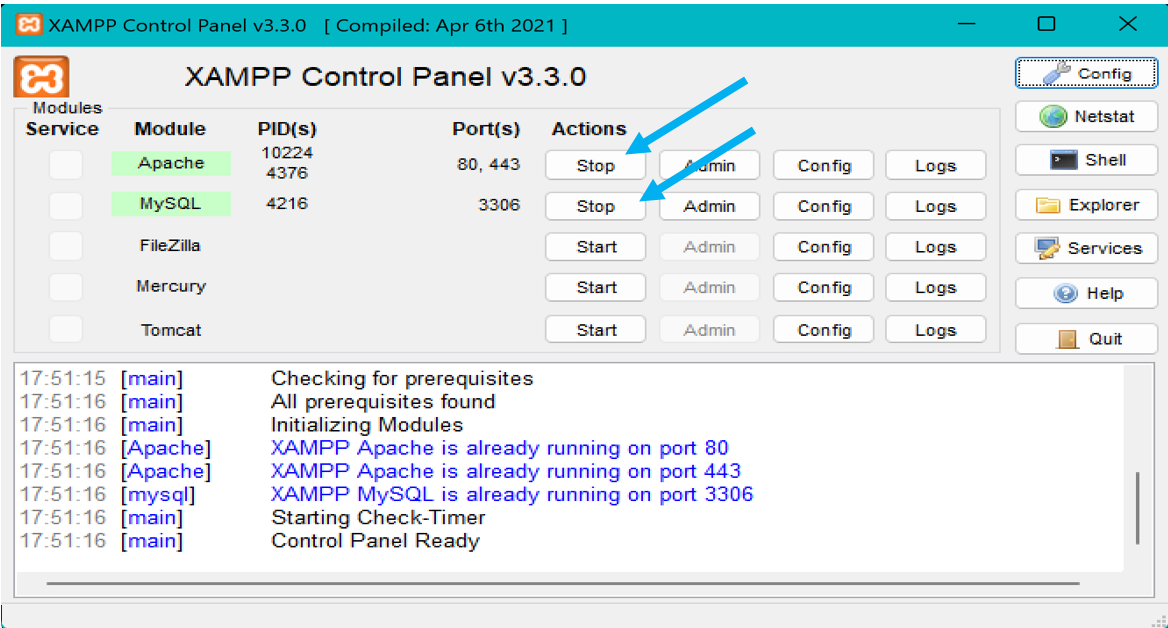
\includegraphics[width=0.75\textwidth]{./img/xampp.png} 
            \caption{Interface XAMPP avec Apache et MySQL activés}
        \end{figure}
\rule{\linewidth}{0.2pt}
    \subsubsection{Créer la base de données sur MySQL}
Une méthode consiste à cliquer sur le bouton "Admin" dans l'onglet MySQL de l’image précédente. Votre navigateur s’ouvrira
automatiquement avec l’adresse suivante dans la barre de recherche :
        \begin{lstlisting}
http://localhost/phpmyadmin/
        \end{lstlisting}
À partir de là, vous pouvez créer votre base de données soit en cliquant sur "Nouvelle base de données" pour effectuer la 
configuration manuellement, soit en saisissant une requête SQL correspondante.
        \begin{figure}[h!] 
            \centering 
            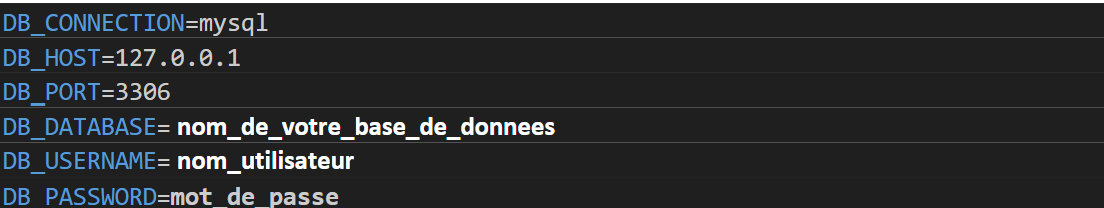
\includegraphics[width=0.95\textwidth]{./img/bd.png} 
            \caption{Interface de phpmyadmin}
        \end{figure}

\rule{\linewidth}{0.2pt}
    \subsubsection{Installer et configurer Elasticsearch} 
-Installation d'Elasticsearch :
\begin{enumerate}

    \item Télécharger Elasticsearch depuis le site officiel.
        \begin{lstlisting}
            elastic.co/downloads/elasticsearch
        \end{lstlisting}
    \item Remplacer le fichier `elasticsearch.yml` selon l'OS.
        \begin{itemize}
            \item Windows :        
Naviguer vers ce dossier dans l'explorateur de fichiers.
Écraser le fichier elasticsearch.yml existant avec le tien (ex. : depuis le dépôt Git).           
            \item Linux :
Si tu l’as installé par archive .tar.gz, le chemin sera similaire à :
        \begin{lstlisting}
            /home/ange_usher/elasticsearch/config/elasticsearch.yml
        \end{lstlisting}
Ou bien si installé en root ou globalement :
        \begin{lstlisting}
            /etc/elasticsearch/elasticsearch.yml
        \end{lstlisting}
Pour le remplacer :
        \begin{lstlisting}
            sudo cp ton_fichier.yml /etc/elasticsearch/elasticsearch.yml
        \end{lstlisting}

        \end{itemize}
    \item Extraire l'archive téléchargée dans un répertoire de votre choix.
        \begin{lstlisting}
Cela reste simple et ne necessite pas un approfondi...
        \end{lstlisting}
    \item Copier le fichier elasticsearch.yml fourni dans le dépôt à l'emplacement de configuration d'Elasticsearch :        
        \begin{itemize}
            \item Windows :
            \begin{lstlisting}
copy config\elasticsearch\elasticsearch.yml C:\chemin\vers\elasticsearch\config\
            \end{lstlisting}
            \item Linux :
            \begin{lstlisting}
/bin/cp config/elasticsearch/elasticsearch.yml /chemin/vers/elasticsearch/config/
            \end{lstlisting}
        \end{itemize}
\end{enumerate}
-Configuration d'Elasticsearch en modifiant le fichier "elasticsearch.yml" :
    \begin{lstlisting}
SCOUT_DRIVER=Matchish\ScoutElasticSearch\Engines\ElasticSearchEngine
ELASTICSEARCH_HOST=http://localhost:9200
ELASTICSEARCH_USER=elastic
ELASTICSEARCH_PASSWORD=changeme
    \end{lstlisting}

\rule{\linewidth}{0.2pt}
    \subsubsection{Lancer Elasticsearch}

Accéder au répertoire d'installation d'Elasticsearch et exécuter :
        \begin{lstlisting}
cd chemin\vers\elasticsearch
# Windows
./bin/elasticsearch.bat
# Linux
./bin/elasticsearch
        \end{lstlisting}

Votre terminal affichera un résultat similaire à :
    \begin{figure}[h] 
        \centering 
        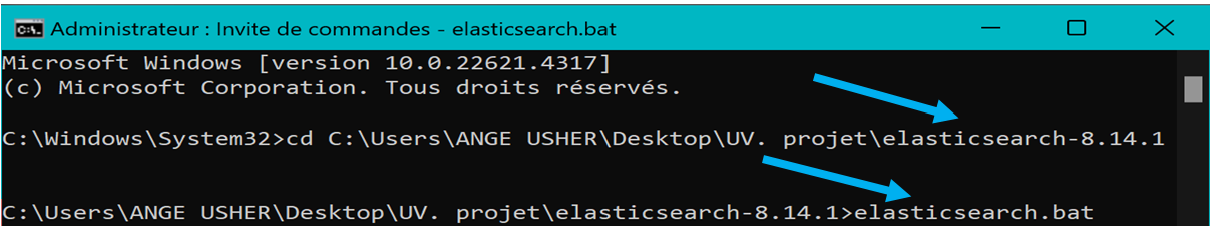
\includegraphics[width=1\textwidth]{./img/elastix.png} 
        \caption{Lancement réussi d'Elasticsearch dans un terminal}
    \end{figure}

\rule{\linewidth}{0.2pt}
    \subsubsection{Lancer le backend Laravel}
Entrer le chemin d’accès au dossier backend dans votre terminal et exécuter :
        \begin{lstlisting}
cd chemin\vers\backend
php artisan migrate:refresh --seed
php artisan serve
        \end{lstlisting}
Vous verrez l'exécution de la commande "php artisan serve" dans votre terminal :
            \begin{figure}[h] 
                \centering 
                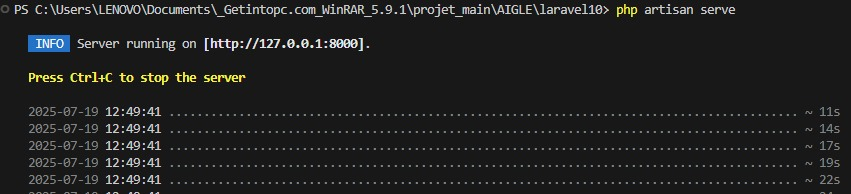
\includegraphics[width=1\textwidth]{./img/back.jpg} 
                \caption{Démarrage du serveur de développement de Laravel (backend)}
            \end{figure}

\rule{\linewidth}{0.2pt}
\newpage
    \subsubsection{Lancer le frontend Angular}
       
Entrer le chemin d’accès au dossier frontend dans votre terminal et exécuter :
        \begin{lstlisting}
cd chemin\vers\frontend
ng serve
        \end{lstlisting}
L'application va commencer à builder et afficher à la fin de l'operation :
            \begin{figure}[h] 
                \centering 
                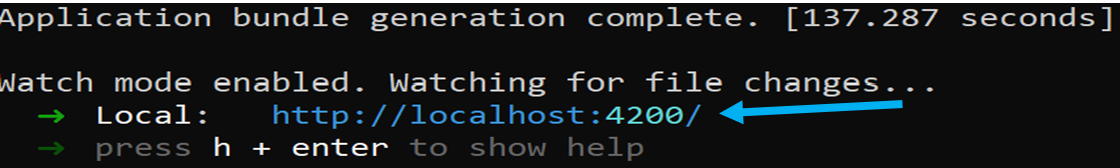
\includegraphics[width=1\textwidth]{./img/angular.png} 
                \caption{Exécution du frontend Angular en local}
            \end{figure}

Accéder à l'application sur :
    \begin{lstlisting}
http://localhost:4200/
    \end{lstlisting}

\vspace{0.5cm}
\vfill
{\fontsize{17}{28}\textbf{\textit{Bienvenue sur l'application AcadProManage :}}}
            \begin{figure}[h] 
                \centering 
                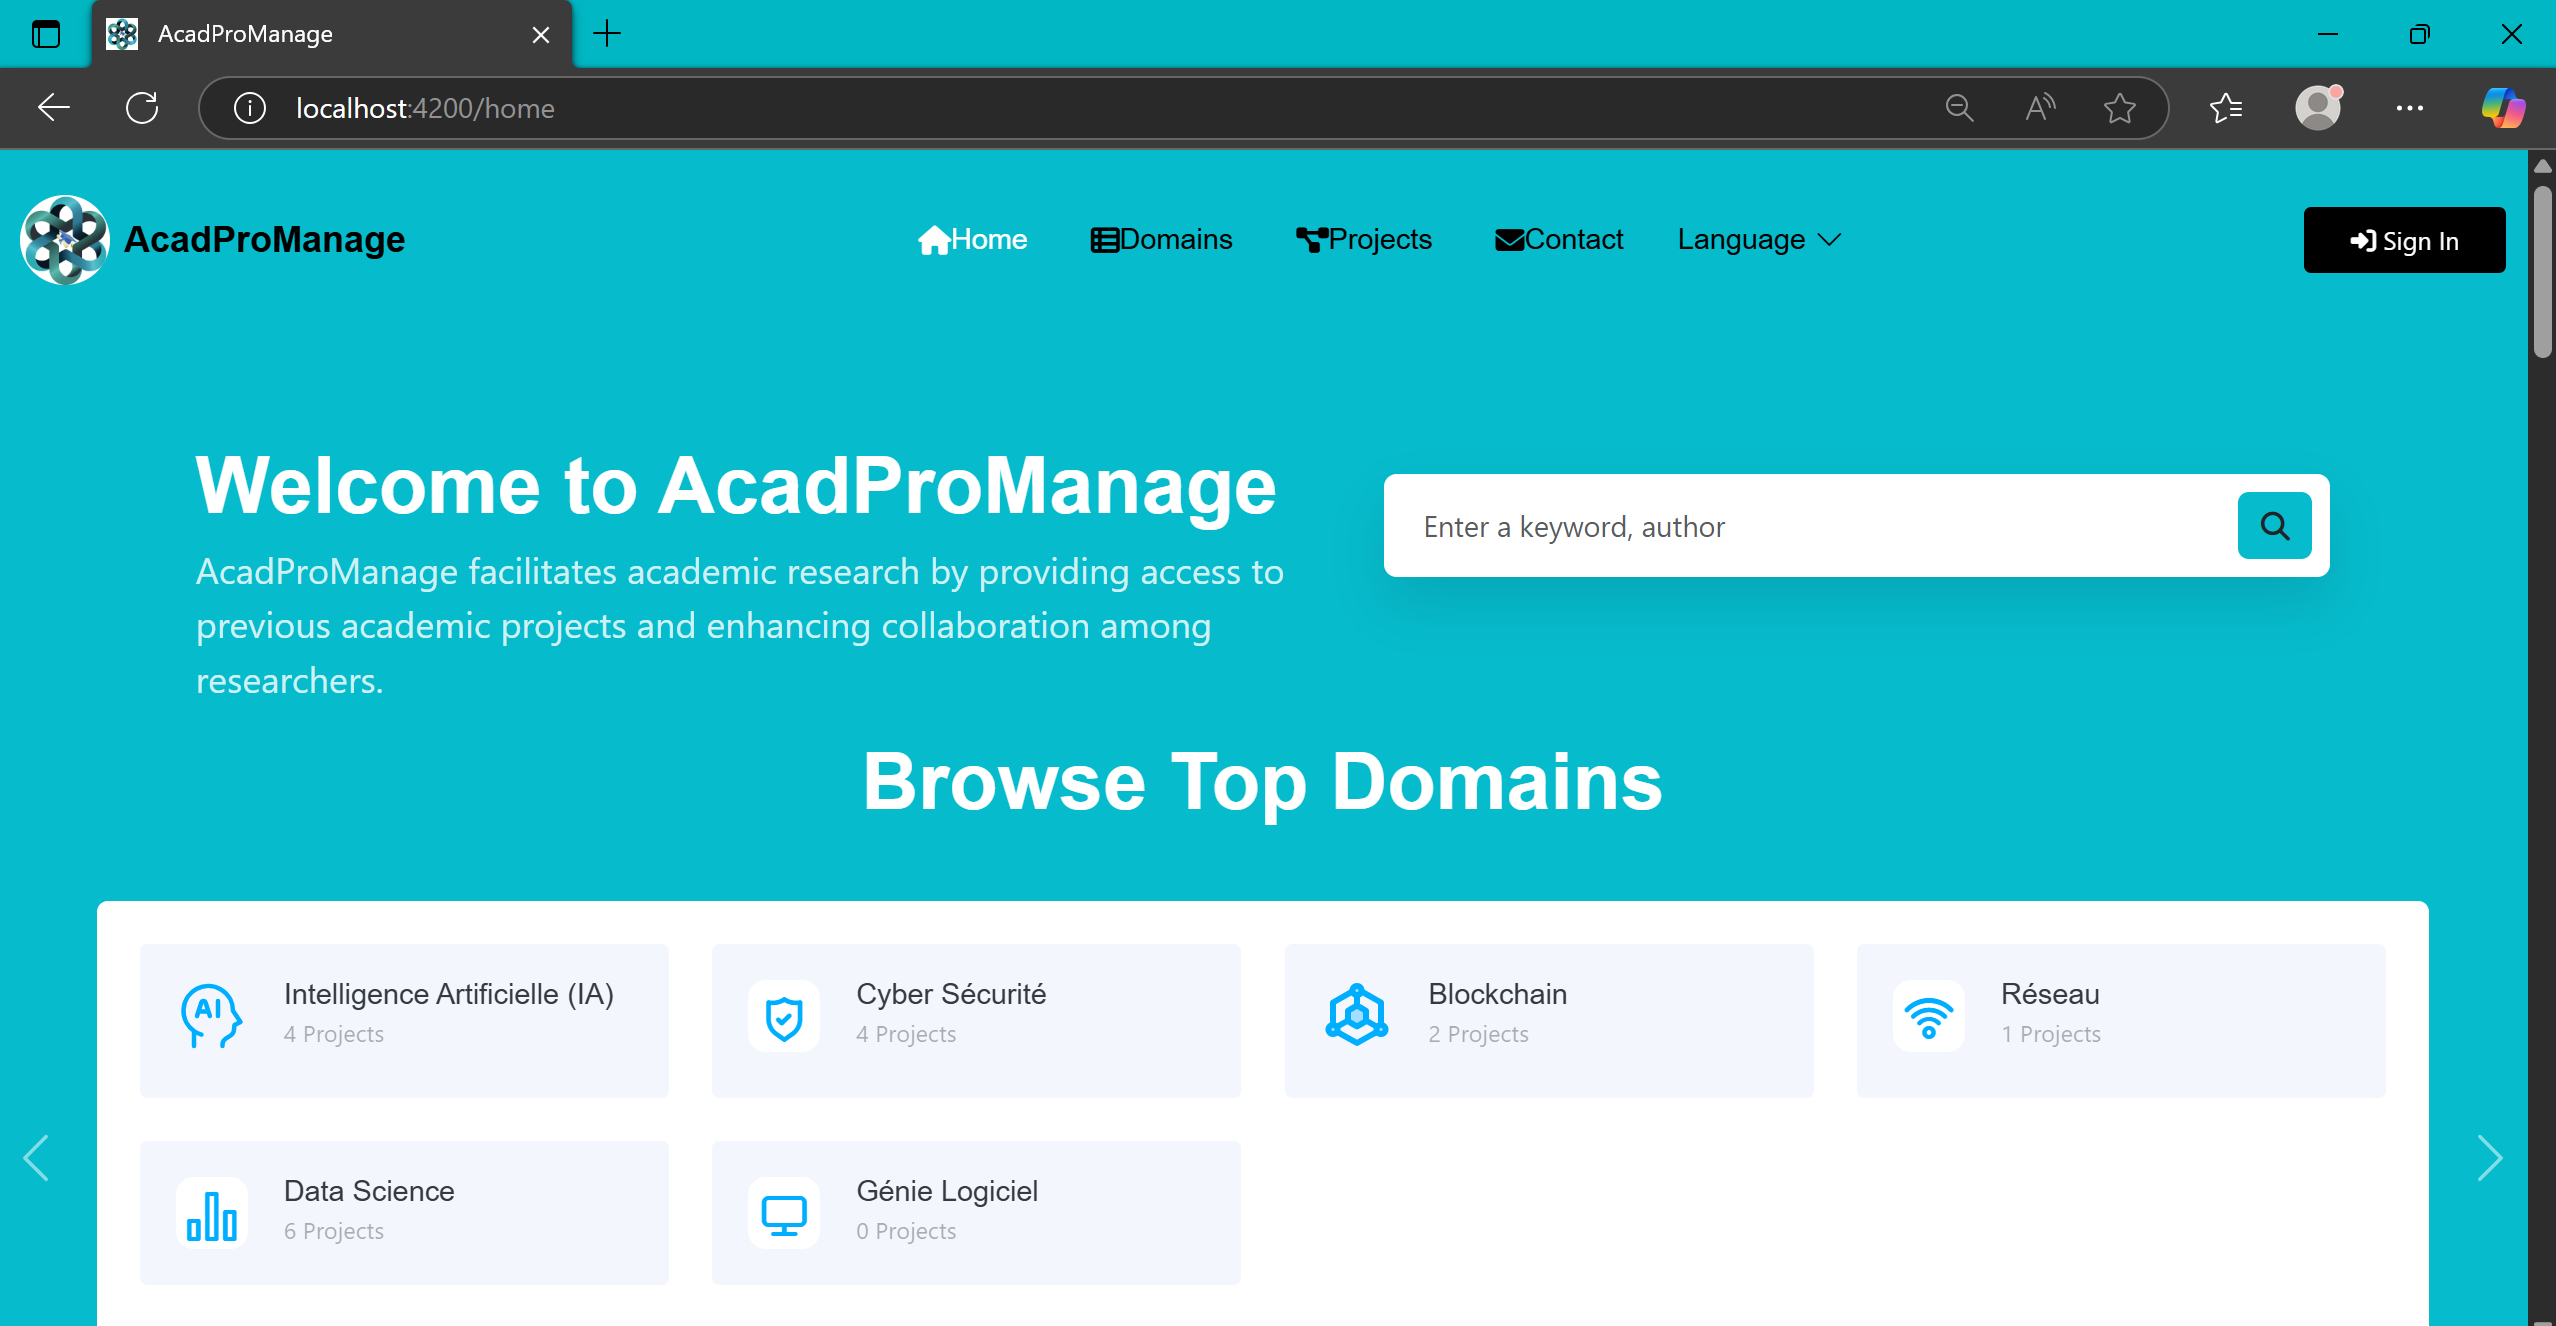
\includegraphics[width=1\textwidth]{./img/ok.png} 
                \caption{Page d'acceuil du projet}
            \end{figure}

\rule{\linewidth}{0.2pt}

\newpage
{\fontsize{14}{16}\textbf{\textit{Problèmes courants :}}}

\begin{itemize}
    \item \textbf{Erreur de connexion à la base de données :} Vérifiez les identifiants dans `.env`.
    \item \textbf{Problème avec Elasticsearch :} Assurez-vous qu’il est bien démarré et que le port est correct.
    \item \textbf{Problème de démarrage de l'application :} Si vous utilisez un antivirus tel que Smadav, désactivez-le 
    temporairement dans le gestionnaire des tâches. En effet, il peut ne pas faire la distinction entre un virus et un 
    programme externe à la machine, ce qui peut empêcher son lancement.
    \item \textbf{Erreur lors de la migration des tables :} Vous devez vous assurez d'avoir installé toutes les dépendances
    requise pour le projet.
\end{itemize}
\rule{\linewidth}{0.2pt}

\newpage
% Conclusion
{\fontsize{14}{16}\section*{Conclusion}}
\addcontentsline{toc}{section}{Conclusion}
En résumé, le processus de déploiement que nous avons détaillé vise à garantir une prise en main claire, structurée 
et pérenne de l'application. En suivant ces étapes, les développeurs et administrateurs actuels comme futurs pourront
assurer la continuité, la maintenance et l’évolution de l’application dans les meilleures conditions.
\end{document}